\documentclass[border=6pt]{standalone}
\usepackage{amsmath}
\usepackage{amssymb}
\usepackage{tikz}
\usepackage{pgfplots}
\pgfplotsset{compat=1.18}
\usetikzlibrary{arrows.meta,calc,positioning}
\begin{document}
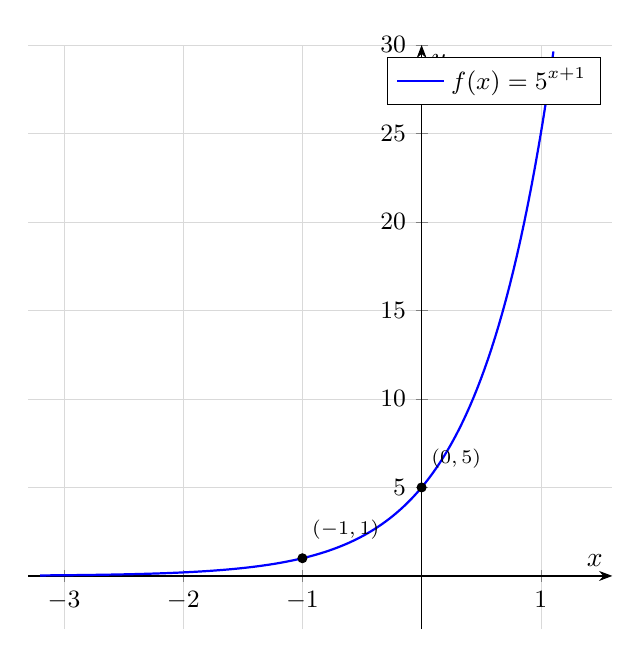
\begin{tikzpicture}
\begin{axis}[
    axis lines = middle,
    xlabel = {$x$}, ylabel = {$y$},
    grid=both,
    grid style={line width=.1pt, draw=gray!30},
    axis line style={-Stealth},
    legend style={font=\small},
    tick label style={font=\small},
    xmin=-3.3, xmax=1.6, ymin=-3, ymax=30,
    xtick={-3,-2,-1,0,1},
    ytick={0,5,10,15,20,25,30},
    width=9cm, height=9cm,
]
\addplot[domain=-3.2:1.35, samples=150, restrict y to domain=-3:30, thick, blue] {5^(x+1)};
\addlegendentry{$f(x)=5^{x+1}$}
\addplot[only marks, mark=*, mark size=1.6pt, black] coordinates {(0,5) (-1,1)};
\node[anchor=south west, font=\scriptsize] at (axis cs:0,5.5) {$(0,5)$};
\node[anchor=south west, font=\scriptsize] at (axis cs:-1,1.5) {$(-1,1)$};
\end{axis}
\end{tikzpicture}
\end{document}
